\documentclass{article}
\usepackage{geometry}
\geometry{a4paper, margin=1in}
\usepackage{graphicx}
\usepackage[colorlinks=true, linkcolor=blue, citecolor=blue, urlcolor=blue]{hyperref}
\usepackage{listings}
\usepackage{xcolor}
\usepackage{amsmath}
\usepackage{enumitem}
\usepackage{float}

\lstset{
    language=NASM,
    basicstyle=\ttfamily\footnotesize\selectfont, % use the selected monospaced font
    backgroundcolor=\color{white},
    keywordstyle=\color{blue},
    commentstyle=\color{gray},
    stringstyle=\color{red},
    numbers=left,
    numberstyle=\tiny\color{gray},
    stepnumber=1,
    numbersep=10pt,
    frame=single,
    breaklines=true,
    captionpos=b,
    tabsize=4
}

\title{Assignment 5: v05 - Display by VRAM as BIOS INT F0}
\author{
    [Welby Seely] \\
    \texttt{[wseely@emich.edu]}
}
\date{\today}

\begin{document}

    \maketitle
    \section{Overview}\label{sec:intro}
    The v4 version of the bootloader was updated to use 0xf0 as an interrupt function group to call the VRAM display function and the VRAM clear function.
    The main refactor was to add the `disp' subroutine with parameter compatibility with BIOS Video Function 0x10 0x13.

    This code is otherwise identical.


    \section{Screenshots}\label{sec:screenshots}
    Screenshots of the splash screen and the prompt screen are provided.

    \begin{figure}[H]  % [H] forces the figure to appear here
        \centering
        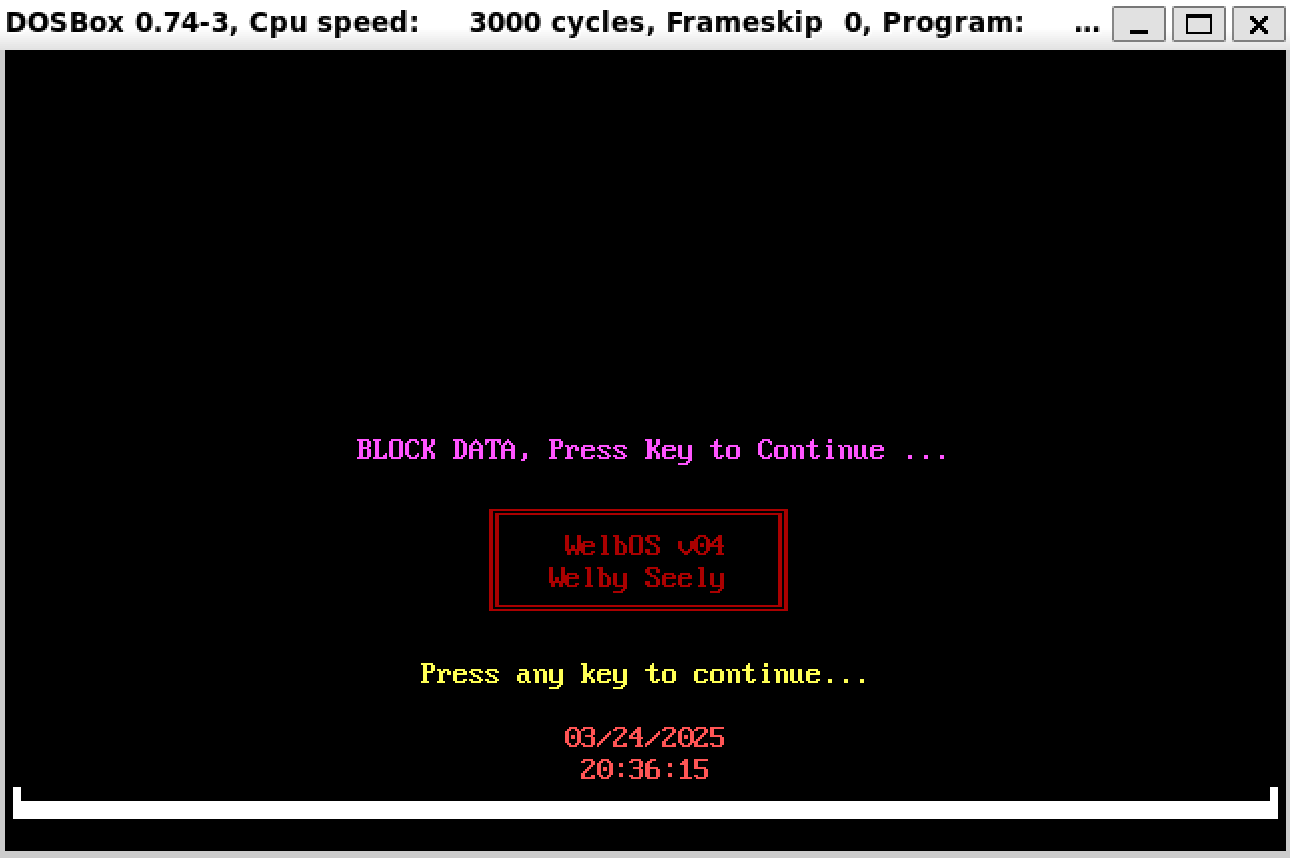
\includegraphics[width=\textwidth]{splash-screen} % Scales image to document width
        \caption{Custom splash screen, complete with block string in the middle}
        \label{fig:1}
    \end{figure}

    \begin{figure}[H]  % Ensures figure appears right here
        \centering
        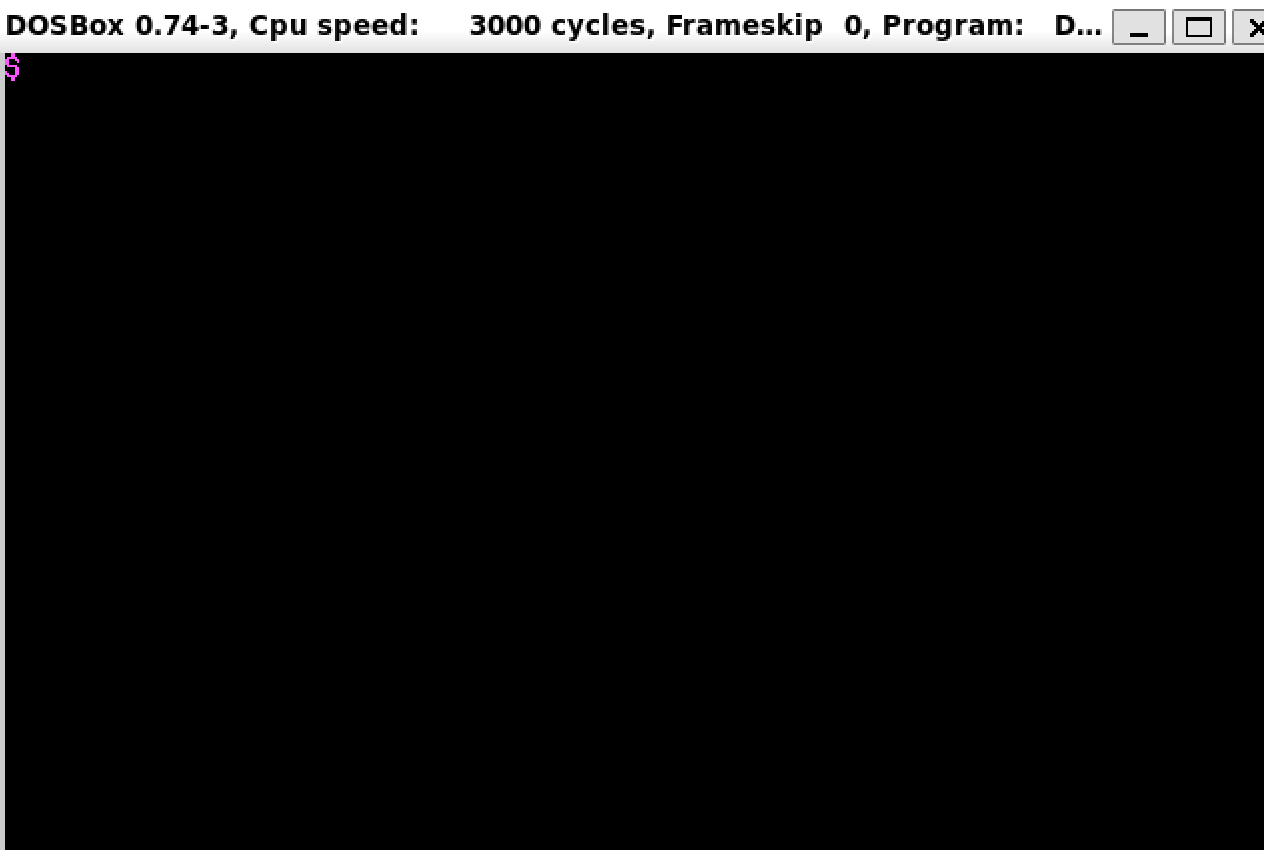
\includegraphics[width=\textwidth]{prompt} % Scales image to document width
        \caption{Prompt with \$ and a blinking cursor}
        \label{fig:2}
    \end{figure}

    \section{Appendix 1: Source Code}\label{sec:appendix_1}
    \begin{lstlisting}[caption={os623V05.asm listing}, captionpos=t]
        bits 16
        BIOS_VIDEO          equ 0x10
        CUSTOM_VIDEO        equ 0xf0
        DISPLAY_FUN         equ 0x13
        CLEAR_FUN           equ 0x06

        BIOS_FLOPPY         equ 0x0013
        READ_SECTORS        equ 0x0002

        ; ext code
        MAIN_SEG equ 0x0001
        MAIN_OFF equ 0x2345

        STRING_SEG equ 0x0001
        STRING_OFF equ 0x7890

        MAGENTA_BLACK equ 0x0D

        ; 1) attribute
        ; 2) length of string
        ; 3) segment of string
        ; 4) address of string
        ; 5) row position
        ; 6) column position
        %macro PRINT 6
            mov bl, %1         ; Attribute (lightgreen on black)
            mov cx, %2         ; length of the string
            mov ax, %3         ; segment of the string
            mov es, ax
            mov bp, %4         ; address of the string
            mov dh, %5         ; row position
            mov dl, %6         ; column position

            mov  ah, DISPLAY_FUN    ; BIOS display string (function 13h)
            mov  al, 0              ; Write mode = 1 (cursor stays after last char
            mov  bh, 0              ; Video page
            int  BIOS_VIDEO
        %endmacro

        org 0x7c00
        jmp short start
        nop

        bsOEM       db "WelbOS v05"         ; OEM String

        start:
            call set_ivt
            ; Inputs: cylinder, sector, head, segment, offset.
            push 1
            push 2
            push 0
            push MAIN_SEG
            push MAIN_OFF

            call 0x:load_sector
            mov ah, CLEAR_FUN
            int CUSTOM_VIDEO

            call MAIN_SEG:MAIN_OFF

            ; Inputs: cylinder, sector, head, segment, offset.
            push 0
            push 2
            push 0
            push 0x0001
            push 0x7890
            call 0x:load_sector

            PRINT MAGENTA_BLACK, 37, 0x0001, 0x7890, 12, 22

            ; Wait for key press
            mov ah, 0x00
            int 0x16

            mov ah, CLEAR_FUN
            int CUSTOM_VIDEO

            push MAGENTA_BLACK
            push 1
            push prompt_sym
            push 0
            push 0
            call 0x:print

            call set_cursor_pos

            int 20h

        set_ivt:
            push ax
            push es

            xor ax, ax
            mov es, ax                                           ; es = 0x0000, IVT segment
            cli                                                  ; disable interrupts during change
            mov word [es:CUSTOM_VIDEO * 4], function_group       ; IP for int 0xf0 → point to `function_group`
            mov   word [es:CUSTOM_VIDEO * 4 + 2 ], cs            ; CS for int 0xf0 → current segment
            sti                                                  ; re-enable interrupts

            pop es
            pop ax
            ret

        times 0x90 - ($ - $$) db 0

        ; -----------------------------------------------------------------------------
        ; Function: print
        ; Description: Prints a string to the console.
        ; Inputs:
        ;   - [bp+6] Column position to begin writing the string.
        ;   - [bp+8] Row position to begin writing the string.
        ;   - [bp+10] Memory address location of the string.
        ;   - [bp+12] Length of the string.
        ;   - [bp+14] Attribute.
        ; Outputs: None.
        ; Modifies:
        ;   - AX, BX, CX, DX, VGA text buffer section (0xB800)

        ; -----------------------------------------------------------------------------
        print:
            push bp
            mov bp, sp
            mov bl, [bp+14]        ; Attribute (lightgreen on black)
            mov cx, [bp+12]        ; length of the string
            push ds
            pop es                 ; segment of the string
            mov dh, [bp+8]         ; row position
            mov dl, [bp+6]         ; column position
            mov bp, [bp+10]        ; address of the string, !!destructive to relative frame refs!!

            mov  ah, 13h            ; BIOS display string (function 13h)
            mov  al, 0              ; Write mode = 1 (cursor stays after last char
            mov  bh, 0              ; Video page
            int CUSTOM_VIDEO

            pop bp
            retf 10

        function_group:
          cmp ah, DISPLAY_FUN
          je .disp
          cmp ah, CLEAR_FUN
          je .clear_screen
          jmp .end

        ; -----------------------------------------------------------------------------
        ; IRQ Function: disp
        ; Description: Prints a string to the console.
        ;    bl         ; Attribute (lightgreen on black)
        ;    cx         ; length of the string
        ;    es:bp      ; address of string
        ;    dh         ; row position
        ;    dl         ; column position
        ; -----------------------------------------------------------------------------
        .disp:
            ; save non-volatile registers
            push ds
            push bx
            push si
            push di

            push bx
            push dx

            push es
            pop ds
            push bp
            pop si

            mov ax, 0xB800
            mov es, ax

            xor ax, ax

            mov al, dh           ; Load row
            mov bx, 80           ; 80 columns per row
            mul bx               ; AX = row * 80

            pop dx
            xor dh, dh
            add ax, dx           ; AX = (row * 80) + column
            shl ax, 1            ; Multiply by 2 (each char = 2 bytes)
            mov di, ax           ; ES:DI now points to VGA memory location

            ; Set up string parameters
            pop bx
            mov ah, bl      ; Attribute byte (foreground/background)

        .write_loop:
            lodsb                ; Load next character from DS:SI into AL
            stosw                ; Store AX (char + attribute) at ES:DI
            loop .write_loop

            pop di
            pop si
            pop bx
            pop ds
            jmp .end

        .clear_screen:
            mov ax, 0xB800      ; Memory-mapped region for text
            mov es, ax
            xor di, di          ; ES:DI = 0xB800:0 (start offset is 0)
            mov ah, 0x07        ; white on black
            mov al, 0x20        ; ASCII space
            mov cx, 2000        ; 80x25 = 2000 characters
            rep stosw           ; Fill screen with spaces and attributes
        .end:
            iret

        times 0x120 - ($ - $$) db 0

        ; -----------------------------------------------------------------------------
        ; Function: load_sector
        ; Description: Loads a sector into memory
        ; Inputs: cylinder, sector, head, segment, offset.
        ; Outputs: 512 bytes into memory as specified by segment and offset.
        ; Note: Does not currently take into account all 10 bits of the cylinder.
        ; Modifies:
        ;   - AX, BX, CX, DX, EX
        ; Calls:
        ;   - BIOS interrupt 0x13, function 0x02.
        ; -----------------------------------------------------------------------------
        load_sector:
            push bp
            mov bp, sp

            mov bx, [bp + 8]            ; segment (can't move immediate into segment register)
            mov es, bx                  ; segment
            mov bx, [bp + 6]            ; offset
            mov ah, READ_SECTORS        ; function
            mov al, 1                   ; number of sectors to read
            mov ch, [bp + 14]           ; cylinder number (10 bits, upper two bits are 6 and 7 of CL)
            mov cl, [bp + 12]           ; sector number (and upper two of cylinder)
            mov dh, [bp + 10]           ; head (usually same as side)
            mov dl, 0                   ; drive number
            int BIOS_FLOPPY

            pop bp
            retf 10

        set_cursor_pos:
            mov ah, 0x01          ; BIOS Set Cursor Shape function
            mov ch, 0x06          ; Start scan line
            mov cl, 0x07          ; End scan line
            int BIOS_VIDEO        ; BIOS video interrupt

            mov ah, 0x02        ; BIOS function: set cursor position
            mov bh, 0x00        ; Page number (0)
            mov dh, 0x00        ; Row (0)
            mov dl, 0x01        ; Column (1)
            int BIOS_VIDEO
            ret

        prompt_sym          db "$"

        ; Pad to 512 bytes for an MBR:
        padding times 510 - ($ - $$) db 0

        ; Optional boot signature:
        bootSig db 0x55, 0xAA

    \end{lstlisting}

    \begin{lstlisting}[caption={loaderV05.asm listing}, captionpos=t]
        bits 16
        BIOS_VIDEO          equ 0x10
        DISPLAY_FUN         equ 0x13

        FUN_VIDEO_MODE      equ 0x0000
        VGA_MODE            equ 0x0003

        BIOS_FLOPPY         equ 0x0013
        READ_SECTORS        equ 0x0002

        VGA_DISPLAY_WIDTH   equ 320
        DISPLAY_WIDTH       equ 80
        DISPLAY_HEIGHT      equ 25
        VGA_TXT_DISP_WIDTH  equ 80
        VGA_TXT_DISP_HEIGHT equ 25
        MESSAGE_ROW         equ VGA_TXT_DISP_HEIGHT / 2 + 3
        LINE_ROW_TOP        equ MESSAGE_ROW - 1
        LINE_ROW_NAME       equ MESSAGE_ROW + 1
        LINE_ROW_BOTTOM     equ LINE_ROW_NAME + 1
        LINE_ROW_ANYKEY     equ LINE_ROW_BOTTOM + 2
        TEXT_MODE           equ 0x03
        MAGENTA_BLACK       equ 0x0D
        WHITE_BLACK         equ 0x0F
        RED_BLACK           equ 0x04
        YELLOW_BLACK        equ 0x0E

        BOX_LENGTH          equ 19
        ANYKEY_LENGTH       equ 28
        BITMAP_LENGTH       equ 18
        SHADE_COUNT         equ 9

        SCALING_FACTOR      equ 0x8
        LOGO_START_X        equ (VGA_DISPLAY_WIDTH - (16 * SCALING_FACTOR)) / 2
        LOGO_START_Y        equ (200 - (9 * SCALING_FACTOR)) / 2 -40

        PRINT_SEGMENT       equ 0
        PRINT_OFFSET        equ 0x7c90

        LOAD_SECTOR_SEGMENT equ 0
        LOAD_SECTOR_OFFSET  equ 0x7d00

        DISPLAY_TIME_SEGMENT equ 0x0002
        DISPLAY_TIME_OFFSET  equ 0x3456

        %define CENTER_TXT(len) ((DISPLAY_WIDTH - len) / 2)
        %define CENTER_VGA_TXT(len) ((VGA_TXT_DISP_WIDTH - len) / 2)

        org 0x2345
        main:
            push ds
            push cs
            pop ds

        hide_cursor:
            mov ah, 0x01          ; BIOS Set Cursor Shape function
            mov ch, 0b00001000    ; Start scan line (set bit 5 to hide cursor)
            mov cl, 0x00          ; End scan line (N/A)
            int BIOS_VIDEO        ; BIOS video interrupt

        load_time:
            push 1
            push 5
            push 0
            push DISPLAY_TIME_SEGMENT
            push DISPLAY_TIME_OFFSET
            call LOAD_SECTOR_SEGMENT:LOAD_SECTOR_OFFSET

            push RED_BLACK
            push BOX_LENGTH
            push welbos
            push MESSAGE_ROW
            push CENTER_VGA_TXT(BOX_LENGTH)
            call PRINT_SEGMENT:PRINT_OFFSET

            push RED_BLACK
            push BOX_LENGTH - 1               ; Repeat count
            push CENTER_VGA_TXT(BOX_LENGTH)   ; Column
            push LINE_ROW_TOP                 ; Row
            push topline                      ; Address of 3-tuple
            call draw_line

            push RED_BLACK
            push BOX_LENGTH
            push name
            push LINE_ROW_NAME
            push CENTER_VGA_TXT(BOX_LENGTH)
            call PRINT_SEGMENT:PRINT_OFFSET

            push RED_BLACK
            push BOX_LENGTH - 1       ; Repeat count
            push CENTER_VGA_TXT(BOX_LENGTH)   ; Column
            push LINE_ROW_BOTTOM     ; Row
            push bottomline             ; Address of 3-tuple
            call draw_line

            push YELLOW_BLACK
            push ANYKEY_LENGTH
            push anykey
            push LINE_ROW_ANYKEY
            push CENTER_VGA_TXT(ANYKEY_LENGTH)
            call PRINT_SEGMENT:PRINT_OFFSET

            push WHITE_BLACK
            push VGA_TXT_DISP_WIDTH - 1       ; Repeat count
            push 0   ; Column
            push LINE_ROW_ANYKEY + 4          ; Row
            push blockline                    ; Address of 3-tuple
            call draw_line

        show_time:
            call DISPLAY_TIME_SEGMENT:DISPLAY_TIME_OFFSET

            pop ds
            retf

        draw_line:
            push bp
            mov bp, sp

            ;left edge
            push word [bp + 12]
            push 1
            mov si, [bp + 4]
            push si
            mov si, [bp + 6]
            push si
            mov si, [bp + 8]
            push si
            call PRINT_SEGMENT:PRINT_OFFSET

            ; set up middle loop
            mov ax, 1                           ; break when == to cx
        draw_line_middle:
            mov cx, [bp + 10]
            cmp ax, cx
            je draw_line_right
            push ax

            push word [bp + 12]
            push 1
            mov si, [bp + 4]
            inc si
            push si
            mov si, [bp + 6]
            push si
            mov si, [bp + 8]
            add si, ax
            push si
            call PRINT_SEGMENT:PRINT_OFFSET

            pop ax
            inc ax
            jmp draw_line_middle

        draw_line_right:
            push word [bp + 12]
            push 1
            mov si, [bp + 4]
            add si, 2
            push si
            mov si, [bp + 6]
            push si
            add ax, [bp + 8]                    ; rightmostposition
            push ax
            call PRINT_SEGMENT:PRINT_OFFSET

            pop bp
            ret 10


        topline             db 0xC9
                            db 0xCD
                            db 0xBB
        bottomline          db 0xC8
                            db 0xCD
                            db 0xBC
        blockline           db 0xDE
                            db 0xDC
                            db 0xDD
        welbos              db 0xBA, `    WelbOS v04   `, 0xBA
        welboslen           equ ($ - welbos)
        name                db 0xBA, `   Welby Seely   `, 0xBA
        namelen             equ ($ - name)
        anykey              db "Press any key to continue..."
        anykeylen           equ ($ - anykey)
    \end{lstlisting}
    \begin{lstlisting}[caption={datetimeV05.asm listing}, captionpos=t]
        PRINT_SEGMENT       equ 0
        PRINT_OFFSET        equ 0x7c90

        VGA_TXT_DISP_HEIGHT equ 25
        VGA_TXT_DISP_WIDTH  equ 80

        MESSAGE_ROW         equ VGA_TXT_DISP_HEIGHT / 2 + 3
        LINE_ROW_TOP        equ MESSAGE_ROW - 1
        LINE_ROW_NAME       equ MESSAGE_ROW + 1
        LINE_ROW_BOTTOM     equ LINE_ROW_NAME + 1
        LINE_ROW_ANYKEY     equ LINE_ROW_BOTTOM + 2
        LIGHT_RED           equ 0x0C

        %macro makedt 4
            mov bh,%1 			;dh/dl/chcl
            shr bh,4
            add bh,30h 			;add 30h to convert to ascii
            mov [%2 + %3],bh
            mov bh,%1
            and bh,0fh
            add bh,30h
            mov [%2 + %4],bh
        %endmacro

        %define CENTER_VGA_TXT(len) ((VGA_TXT_DISP_WIDTH - len) / 2)

        bit16
        org 0x3456

            push ds
            push cs
            pop ds

            mov ah,04h	 ;function 04h (get RTC date)
            int 1Ah		;BIOS Interrupt 1Ah (Read Real Time Clock)

            makedt dh, dtfld, 0, 1  ; month
            makedt dl, dtfld, 3, 4  ; day
            makedt ch, dtfld, 6, 7  ; century
            makedt cl, dtfld, 8, 9  ; year

            mov ah,02h
            int 1Ah

            makedt ch, tmfld, 0, 1  ; hours
            makedt cl, tmfld, 3, 4  ; minutes
            makedt dh, tmfld, 6, 7  ; seconds

            push LIGHT_RED
            push 10
            push dtfld
            push LINE_ROW_ANYKEY + 2
            push CENTER_VGA_TXT(10)
            call PRINT_SEGMENT:PRINT_OFFSET

            push LIGHT_RED
            push 8
            push tmfld
            push LINE_ROW_ANYKEY + 3
            push CENTER_VGA_TXT(8)
            call PRINT_SEGMENT:PRINT_OFFSET

            pop ds
            retf

        dtfld: db '00/00/0000'
        tmfld: db '00:00:00'

    \end{lstlisting}

    \begin{lstlisting}[caption={stringV05.asm listing}, captionpos=t]
        db 'BLOCK DATA, Press Key to Continue ...'
    \end{lstlisting}
    \end{document}
